\chapter{Application of GRAPE: Robust Control for Transmon}
\label{chap:robust}

This chapter turns to a concrete application of GRAPE: the design of detuning-robust control pulses for transmon gates. The transmon has been widely used as either a qubit or an ancilla for bosonic qubits. In both cases, the $\hat{X}_\theta$ gate in the first two-level subspace of the transmon is crucial for realizing universal gates in the composite system. One important preliminary to obtaining high-fidelity gates in the composite system is to acquire a robust $\hat{X}_\theta$ in the single-transmon system.

Detuning-robust control for two-level systems has been extensively investigated using various approaches, including reverse engineering~\cite{PhysRevLett.111.050404inverseengi,PhysRevLett.125.250403inverseengi}, space curve quantum control~\cite{barnes2022dynamicallyspacecurve}, pulse engineering~\cite{barnes2022dynamicallyspacecurve,wang2012compositepulse,PhysRevA.83.053420pulse,PhysRevA.86.022315pulse,tycko1983broadbandpulse,PhysRevA.107.023103pulse,ball2021softwarepulseengi,wimperis1994broadbandpulse,pasini2009optimizedinitialpulse}, and the collocation method~\cite{propson2022robustcollocation,Trowbridge2023}. However, protocols developed for two-level systems cannot be directly applied to weakly anharmonic transmons due to leakage out of the qubit subspace. One promising solution is to apply the DRAG scheme to robust single-quadrature pulses developed for two-level systems~\cite{hai2023universalcompare}. 
Additionally, Ref.~\cite{qctrl} directly optimizes two-quadrature pulses for transmons.
In the following, I introduce an alternative optimization-based procedure to design detuning-robust control for transmon $\hat{X}_{\theta}$ gates and benchmark its performance.

\section{Metrics of robust control}
\label{sec:metrics}

During the gate operation, the Hamiltonian of interest may depend on an unknown quantity $\delta$. This uncertainty can cause the realized gate to deviate from the target gate, thus generally lowering gate fidelity $\mathcal{I}(\delta)$. To quantify the robustness of the infidelity against $\delta$, I consider both the mean infidelity and its standard deviation as key metrics,
\begin{equation}
\label{eq:robust_metrics}
\mathcal{I}_\mu = \int_\mathbb{D} \mathrm{d}\delta\, p(\delta)\mathcal{I}(\delta), \quad
\mathcal{I}_\sigma =\sqrt{\int_\mathbb{D} \mathrm{d}\delta \, p(\delta)\big[\mathcal{I}(\delta)-I_\mu\big]^2 }.
\end{equation}
Here, the probability distribution $p(\delta)$ satisfies $\int_\mathbb{D}\mathrm{d}\delta \, p(\delta)=1$ for a specified range $\mathbb{D}$. 

In the case of interest, the Hamiltonian governing the transmon qubit in the co-rotating frame of the drive frequency is 
\begin{equation}
\label{eq:H_trans}
    \hat{H}_\text{trans}(t) = K_\text{q} \hat{q}^{\dagger 2} \hat{q}^2/2 + \varepsilon_I(t)(\hat{q}^\dagger+\hat{q})+i\varepsilon_Q(t)(\hat{q}^\dagger-\hat{q})+\delta \hat{q}^\dagger \hat{q}.
\end{equation}
Here, $\varepsilon_I(t)$ and $\varepsilon_Q(t)$ describe control envelopes in the $I$ and $Q$ quadratures, and $\delta$ denotes the difference between the drive frequency and the unknown shifted qubit frequency.%
\nomenclature{$\varepsilon_I$, $\varepsilon_Q$}{Control envelopes in the $I$ and $Q$ quadratures}%
\nomenclature{$K_\text{q}$}{Transmon anharmonicity (self-Kerr)}%
The closed-system gate infidelity follows 
\begin{equation}\label{eq:fid_single}
\mathcal{I}_\text{c}(\delta) = 1-\frac{1}{4}\left|\Tr\left[\hat{P}_{0,1}\hat{U}_\text{target}^\dagger \hat{U}_\delta(t_\text{g})\right]\right|^2,
\end{equation}
where $\hat{P}_{0,1}$ is a projector onto the computational subspace formed by the lowest two eigenstates. Here, $\hat{U}_\text{target}$ is the target unitary on the transmon, and $\hat{U}_\delta(t_\text{g})=\mathcal{T}\exp[-i\int_0^{t_\text{g}} \mathrm{d}\tau \, \hat{H}_\text{trans}(\tau)]$ is the actual unitary achieved over a gate duration $t_\text{g}$, where $\mathcal{T}$ is the time-ordering operator. 

In the presence of decoherence, the open-system infidelity follows~\cite{abdelhafez2019quantumthesis}
\begin{equation}
\label{eq:open_inf}
\mathcal{I}_\text{o}(\delta) = 1-\frac{1}{4}\Tr[\mathcal{P}_{0,1}\mathcal{L}_\text{target}^\dagger \mathcal{L}_\delta(t_\text{g})].
\end{equation}
Here, the density matrix is vectorized by stacking the elements row-by-row. $\mathcal{P}_{0,1}=\hat{P}_{0,1}\otimes\hat{P}_{0,1}$ is the superprojector onto the computational subspace, $\mathcal{L}_\text{target}=\hat{U}_\text{target}\otimes \hat{U}^*_\text{target}$ is the target superoperator, and $\mathcal{L}_\delta(t_\text{g})$ is the superoperator realized by the Lindblad master equation. Note that in the absence of decoherence, $\mathcal{L}_\delta(t_\text{g})=\hat{U}_\delta(t_\text{g})\otimes \hat{U}_\delta^*(t_\text{g})$.

\section{Optimization procedure}
\label{sec:opt_procedure}

Quantum optimal control has been extensively used to develop robust control schemes by minimizing cost functions that encode robustness metrics. One approach is to penalize the derivative of the closed- or open-system fidelity with respect to detuning $\delta$~\cite{Watanabe,hai2023universalcompare,qctrl}. However, a more intuitive and pragmatic method is to penalize the average infidelity~\cite{reinhold2019controllingthesisrobustmetric,allen2020robustmetric,kosut2013robustmetric,khaneja2005optimalrobustmetric,rembold2020introductionrobustmetric}
\begin{equation}\label{eq:avg_inf}
C_{\text{o},\text{c}} = \frac{1}{N}\sum_{i=1}^N\mathcal{I}_{\text{o},\text{c}}(\delta_i).
\end{equation}
Here, $\delta_i$ denotes sample values of detunings within the specified range of $\mathbb{D}$. Minimization of the above cost function can suppress both mean infidelity and its standard deviation, as evidenced by the subsequent numerical results.

\begin{figure}[t]
    \centering
    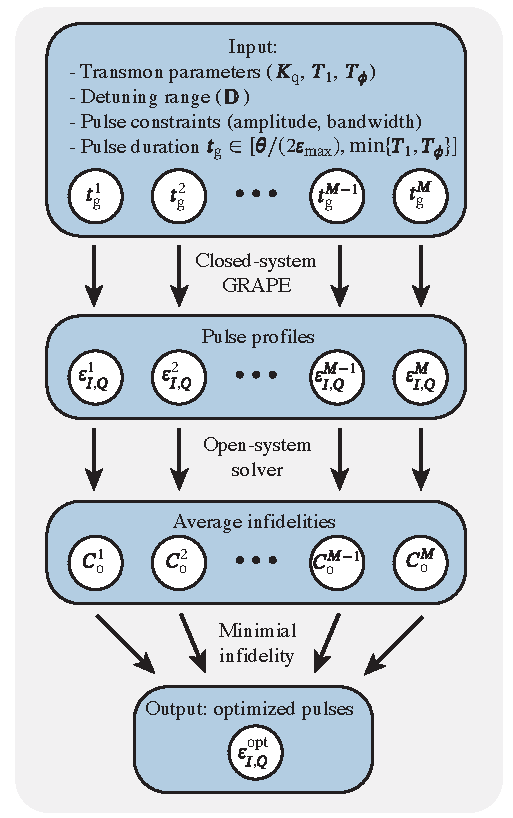
\includegraphics[width=0.7\linewidth]{ch4_figures/fig_flowchart.pdf}
    \caption[Optimization procedure to obtain detuning-robust $\hat{X}_\theta$ gates in transmons.]{
    Optimization procedure to obtain detuning-robust $\hat{X}_\theta$ gates in transmons. Input includes pulse constraints, transmon parameters, and a set of $M$ pulse durations. The choice of duration should be shorter than the decay time $T_1$ and longer than $1/\varepsilon_\text{max}$, where $\varepsilon_\text{max}$ is the maximum pulse amplitude. Closed-system GRAPE is performed for each duration to obtain the corresponding pulse profiles. Subsequently, an open-system solver evaluates the cost function $C_\text{o}$ for pulses with varying durations, selecting the pulse that minimizes $C_\text{o}$.}
    \label{fig:optflow}
\end{figure}

To minimize the cost function, I optimize the pulses, including both the envelopes $\varepsilon_{I,Q}(t)$ and the pulse duration $t_\text{g}$. 
An optimal duration is determined by balancing two competing factors: a shorter duration leads to unwanted leakage, whereas a longer duration results in decoherence errors. 
A direct approach to optimize pulses involves using an open-system optimizer for various durations and selecting the one that minimizes the cost function $C_\text{o}$. 
However, such optimization requires time-intensive open-system simulations. 
Instead, I propose a method that, while not guaranteed to be equivalent, yields promising results. 
The method consists of two steps: (1)~employing closed-system optimization to minimize $C_\text{c}$ for each potential duration, and (2)~with given decoherence rates, evaluating $C_\text{o}$ for the optimized pulses from the first step, then selecting the pulse with the lowest $C_\text{o}$. 
The approach is summarized in Fig.~\ref{fig:optflow}.

For the closed-system optimization, I use Gradient Ascent Pulse Engineering (GRAPE), a method widely employed for optimal control in various contexts~\cite{khaneja2005optimalrobustmetric,lu2023optimalgrape,koch2022quantumqocreview}. The gradients required in GRAPE are calculated by using automatic differentiation, thereby eliminating the need for manually coding the analytical gradients of the cost function~\cite{adscalingbaydin2014automatic,PhysRevA.95.042318ad,PhysRevA.99.052327ad}. The initial pulse ansatz is
\begin{align}
\label{eq:initial_pulse}
    \varepsilon^\text{initial}_I(t) &=\frac{1}{t_\text{g}}\big[ (a-\theta/2)\cos(2\pi t /t_\text{g}) + (b-a)\cos(4\pi t /t_\text{g})\\ 
\nonumber     &+(c-b)\cos(6\pi t / t_\text{g}) - c\cos(8\pi t / t_\text{g}) + \theta/2\big],\\
\nonumber    \varepsilon_Q^\text{initial}(t) & = -\dot{\varepsilon}_I^\text{initial}(t) / K_\text{q},
\end{align}
where $\theta$ is the rotation angle for the target $\hat{X}_\theta$ gate ($\theta=\pi,\pi/2$ in this study). This ansatz for the $I$-quadrature control has been used to obtain robust control for two-level systems~\cite{pasini2009optimizedinitialpulse}. The initial guess for the $Q$-quadrature is inspired by the DRAG pulse scheme~\cite{Motzoi2009} to suppress leakage. 
The pulse is then optimized starting from various initial guesses for parameters $a,b,c\in\{-10,-8,-6,\cdots,10\}$, and the pulse with the lowest cost value $C_\text{c}$ is selected. This process is accelerated by parallelizing with different initial values.

Throughout the closed-system optimization process, I ensure pulse smoothness by filtering out frequency components that exceed maximum allowed bandwidths of $5/t_\text{g}$ and $10/t_\text{g}$ for $\varepsilon_I(t)$ and $\varepsilon_Q(t)$, respectively. These empirical values effectively balance pulse smoothness and the level of robustness required.

\section{Benchmarking and comparison}
\label{sec:benchmarking}

\begin{figure}[t]
    \centering
    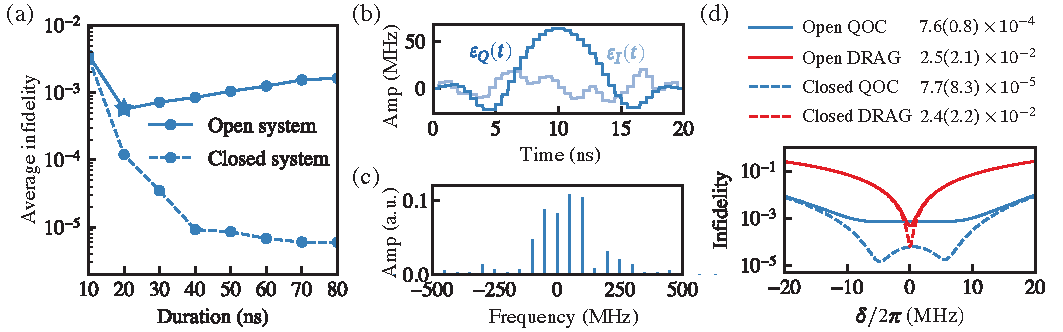
\includegraphics[width=\textwidth]{ch4_figures/fig_qoc.pdf}
    \caption[Optimization results for the $\hat{X}_\pi$ gate.]{
    Optimization results for the $\hat{X}_\pi$ gate. 
(a)~Average infidelities in Eq.~\eqref{eq:avg_inf} versus pulse durations for both closed (dashed line) and open (solid line) systems. The optimal duration selected from the range considered for this optimization is 20\,ns (indicated by a star). 
(b)~$I$ and $Q$ quadratures of the pulse envelopes for the selected 20-ns pulse from~(a).
(c)~The frequency components of the pulse envelopes, corresponding to the 20-ns pulse. 
(d)~Comparative analysis of the 20-ns pulses, from both QOC (blue) and DRAG (red) pulses, in terms of their infidelities as a function of detuning.
The average and standard deviation of the infidelities are tabulated correspondingly by considering a uniform distribution of $\rho(\delta)$ for simplicity. The result shows that the optimized pulse is more robust than the commonly used DRAG pulse.
[Parameters: $\delta_i/2\pi\in\{\pm 1,\pm 3,\pm 4,\pm 7,\pm 10\}$\,MHz, $K_\text{q}/2\pi=-200$\,MHz, $T_1=50$\,$\mu$s, $T_\phi=50$\,$\mu$s.]}
    \label{fig:fig_qoc}
\end{figure}

I benchmark the optimization procedure for a transmon with typical parameters: $K_\text{q}/2\pi=-200$\,MHz, $T_1=50$\,$\mu$s, and $T_\phi=50$\,$\mu$s. The optimization results for the $\hat{X}_\pi$ gate are shown in Fig.~\ref{fig:fig_qoc}. 
Figure~\ref{fig:fig_qoc}(a) shows the average infidelities obtained for closed- and open-system simulations with varying pulse durations. 
Without decoherence, extending the pulse duration generally leads to a reduction in the cost value. In contrast, in the presence of decoherence, utilizing shorter pulses is more effective in reducing the infidelity. 
Given the particular transmon parameters under consideration, a pulse duration of 20\,ns achieves the lowest cost.
The temporal profiles and frequency components of the optimized 20-ns pulse are shown in Fig.~\ref{fig:fig_qoc}(b) and~(c), respectively.
In Fig.~\ref{fig:fig_qoc}(d), the infidelity as a function of detuning is studied, comparing the performance between the optimized and the DRAG pulses. 
In both closed- and open-system simulations, the optimized pulse consistently demonstrates substantially reduced infidelities across almost all detunings. 
Consequently, the optimized pulse exhibits enhanced robustness against frequency detuning in the transmon ancilla. 
The open-system infidelities obtained from these two pulses are limited by distinct factors: the infidelity derived from the QOC pulse is dominated by decoherence errors, while the one generated from the DRAG pulse is limited by coherent error. 

\begin{figure}[t]
    \centering
    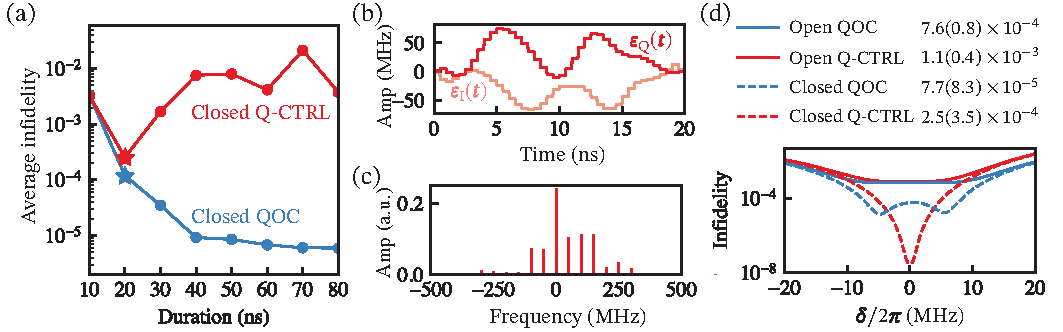
\includegraphics[width=\textwidth]{ch4_figures/fig_qoc_qctrl.pdf}
    \caption[Comparison of optimization results between Q-CTRL and QOC for the $\hat{X}_{\pi}$ gate.]{
Comparison of optimization results between Q-CTRL and QOC for the $\hat{X}_{\pi}$ gate.
(a)~Average infidelities of a closed system [Eq.~\eqref{eq:avg_inf}] versus pulse durations derived from Q-CTRL (red) and QOC (blue). The optimal duration selected for Q-CTRL from the range considered is 20\,ns (indicated by a red star).
(b)~$I$ and $Q$ quadratures of the Q-CTRL pulse envelopes for the selected 20-ns pulse from~(a).
(c)~Frequency components of the Q-CTRL pulse envelopes corresponding to the 20-ns pulse.
(d)~Comparative analysis of the 20-ns pulses from both QOC (blue) and Q-CTRL (red) in terms of their infidelities as a function of detuning.
The average and standard deviation of the infidelities are tabulated considering a uniform distribution of $\rho(\delta)$ for simplicity.
[Parameters: $\delta_i/2\pi \in \{\pm 1, \pm 3, \pm 4, \pm 7, \pm 10\}$\,MHz, $K_\text{q}/2\pi = -200$\,MHz, $T_1 = 50$\,$\mu$s, $T_\phi = 50$\,$\mu$s.]}
    \label{fig:fig_qoc_qctrl}
\end{figure}

I then compare the robustness of the pulses derived from this optimization procedure with selected recent literature. First, following the methodology outlined in Ref.~\cite{qctrl}, I obtain robust pulses using the \texttt{Q-CTRL} package~\cite{ball2021softwarepulseengi,qctrl2022boulder}. To distinguish between these results and those generated by the optimization procedure presented here, I use the label ``Q-CTRL'' for the former and ``QOC'' for the latter.
The averaged infidelities [Eq.~\eqref{eq:avg_inf}] of the closed system as a function of pulse duration are shown in Fig.~\ref{fig:fig_qoc_qctrl}(a). While the average infidelities for Q-CTRL (red) and QOC (blue) are similar for shorter durations, QOC demonstrates orders of magnitude lower infidelity for longer durations. To illustrate the robustness details of the Q-CTRL results, I examine the 20-ns case, which exhibits the lowest infidelity. The $I$ and $Q$ quadratures of the pulse envelopes and their corresponding Fourier components are shown in Fig.~\ref{fig:fig_qoc_qctrl}(b) and~(c). The infidelity as a function of detuning is presented in Fig.~\ref{fig:fig_qoc_qctrl}(d).
For a closed system, the Q-CTRL results (red dashed line) show lower infidelity near resonance but exhibit higher infidelity off-resonance ($\delta/2\pi > 5$\,MHz) compared to the QOC results (blue dashed line). This difference likely arises from the different cost functions used in the two optimizations: Q-CTRL penalizes the derivative of the infidelity at zero detuning, whereas QOC minimizes the average infidelity over a sampling of detunings ($\delta_i/2\pi \in \{\pm 1, \pm 3, \pm 4, \pm 7, \pm 10\}$\,MHz in this example). Notably, in the presence of ancilla decoherence ($T_1 = 50$\,$\mu$s, $T_\phi = 50$\,$\mu$s), the infidelity at small detuning is dominated by incoherent error. This makes QOC the overall better choice within the considered range of detuning for robust pulses.

The results of this chapter demonstrate that the GRAPE-based optimization procedure developed here generates detuning-robust transmon pulses that outperform both conventional DRAG pulses and Q-CTRL pulses across the relevant detuning range.
